% Linked-list schematic for the L3b lecture. Completes the 2/4/8/16 motif of
% Fig-Stack.svg and Fig-Queue.svg: the stack pushed 16 on top, the queue added
% it at the back, and the linked list splices it into the middle.
%
% Build (from this directory):
%   pdflatex Fig-LinkedList.tex
%   pdf2svg Fig-LinkedList.pdf Fig-LinkedList.svg
%   then re-add the accessibility title element after the opening <svg> tag:
%   <title>Linked list</title>
\documentclass[tikz,border=10pt]{standalone}
\usetikzlibrary{arrows.meta, calc}
\definecolor{chemered}{HTML}{EF4035}
\definecolor{chemewheat}{HTML}{FAEEE2}
\begin{document}
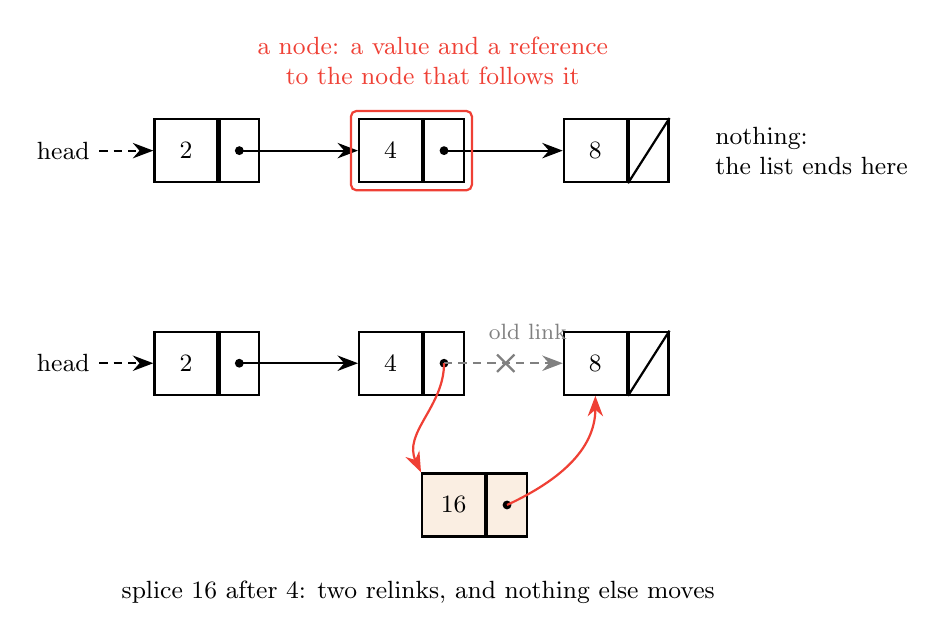
\begin{tikzpicture}[
    vbox/.style={draw=black, thick, minimum width=8mm, minimum height=8mm, inner sep=1pt, font=\small},
    pbox/.style={draw=black, thick, minimum width=5mm, minimum height=8mm, inner sep=0pt},
    note/.style={font=\small, align=left},
    ref/.style={-{Stealth[length=2.6mm]}, thick},
    headref/.style={-{Stealth[length=2.6mm]}, thick, dash pattern=on 3pt off 2.2pt},
    x=1cm, y=1cm]

    % ================= row 1: the list =================
    \node[note, anchor=east] (head) at (-1.1, 0) {head};

    \node[vbox] (a)  at (0, 0) {$2$};
    \node[pbox, anchor=west] (ap) at (a.east) {};
    \node[vbox] (b)  at (2.6, 0) {$4$};
    \node[pbox, anchor=west] (bp) at (b.east) {};
    \node[vbox] (c)  at (5.2, 0) {$8$};
    \node[pbox, anchor=west] (cp) at (c.east) {};

    % the head references the first node; each node references the next -
    \draw[headref] (head) -- (a.west);
    \fill (ap.center) circle (1.6pt);
    \draw[ref] (ap.center) -- (b.west);
    \fill (bp.center) circle (1.6pt);
    \draw[ref] (bp.center) -- (c.west);

    % the last node references nothing -
    \draw[thick] (cp.south west) -- (cp.north east);
    \node[note, anchor=west] at (6.6, 0) {nothing:\\the list ends here};

    % a node is a value plus a reference -
    \draw[thick, chemered, rounded corners=2pt]
        ($(b.south west)+(-0.09,-0.09)$) rectangle ($(bp.north east)+(0.09,0.09)$);
    \node[note, text=chemered, align=center, anchor=south] at ($(b.north east)+(0.12,0.30)$)
        {a node: a value and a reference\\to the node that follows it};

    % ================= row 2: the splice =================
    \node[note, anchor=east] (head2) at (-1.1, -2.7) {head};

    \node[vbox] (a2)  at (0, -2.7) {$2$};
    \node[pbox, anchor=west] (a2p) at (a2.east) {};
    \node[vbox] (b2)  at (2.6, -2.7) {$4$};
    \node[pbox, anchor=west] (b2p) at (b2.east) {};
    \node[vbox] (c2)  at (5.2, -2.7) {$8$};
    \node[pbox, anchor=west] (c2p) at (c2.east) {};

    \draw[headref] (head2) -- (a2.west);
    \fill (a2p.center) circle (1.6pt);
    \draw[ref] (a2p.center) -- (b2.west);
    \fill (b2p.center) circle (1.6pt);
    \draw[thick] (c2p.south west) -- (c2p.north east);

    % the old link from 4 to 8 is retired: grayed out and crossed -
    \draw[ref, gray, dash pattern=on 3pt off 2.2pt] (b2p.center) -- (c2.west);
    \coordinate (oldmid) at ($(b2p.center)!0.52!(c2.west)$);
    \draw[thick, gray] ($(oldmid)+(-0.11,-0.11)$) -- ($(oldmid)+(0.11,0.11)$);
    \draw[thick, gray] ($(oldmid)+(-0.11,0.11)$) -- ($(oldmid)+(0.11,-0.11)$);
    \node[note, gray, anchor=south, font=\footnotesize] at ($(oldmid)+(0.28,0.18)$) {old link};

    % the new node, spliced in with two relinks and no shifting -
    \node[vbox, fill=chemewheat] (m)  at (3.4, -4.5) {$16$};
    \node[pbox, anchor=west, fill=chemewheat] (mp) at (m.east) {};
    \fill (mp.center) circle (1.6pt);
    \draw[ref, chemered] (b2p.center) to[out=-90, in=115] (m.north west);
    \draw[ref, chemered] (mp.center) to[out=25, in=-90] (c2.south);

    % caption, centered under the action -
    \node[note, align=center, anchor=north] at (2.95, -5.35)
        {splice $16$ after $4$: two relinks, and nothing else moves};
\end{tikzpicture}
\end{document}
